\documentclass{article}
\usepackage{polski} %moze wymagac dokonfigurowania latexa, ale jest lepszy niż standardowy babel'owy [polish] 
\usepackage[utf8]{inputenc} 
\usepackage[OT4]{fontenc} 
\usepackage{graphicx,color} %include pdf's (and png's for raster graphics... avoid raster graphics!) 
\usepackage{url} 
\usepackage[pdftex,hyperfootnotes=false,pdfborder={0 0 0}]{hyperref} %za wszystkimi pakietami; pdfborder nie wszedzie tak samo zaimplementowane bo specyfikacja nieprecyzyjna; pod miktex'em po prostu nie widac wtedy ramek


% Zmiana rozmiar�w strony tekstu
\addtolength{\voffset}{-1cm}
\addtolength{\hoffset}{-1cm}
\addtolength{\textwidth}{2cm}
\addtolength{\textheight}{2cm}

%bardziej zyciowe parametry sterujace rozmieszczeniem rysunkow
\renewcommand{\topfraction}{.85}
\renewcommand{\bottomfraction}{.7}
\renewcommand{\textfraction}{.15}
\renewcommand{\floatpagefraction}{.66}
\renewcommand{\dbltopfraction}{.66}
\renewcommand{\dblfloatpagefraction}{.66}
\setcounter{topnumber}{9}
\setcounter{bottomnumber}{9}
\setcounter{totalnumber}{20}
\setcounter{dbltopnumber}{9}

% w�asny bullet list z malymi odstepami
\newenvironment{tightlist}{
\begin{itemize}
  \setlength{\itemsep}{1pt}
  \setlength{\parskip}{0pt}
  \setlength{\parsep}{0pt}}
{\end{itemize}}




%\title{Sprawozdanie z laboratorium:\\Metaheurystyki i Obliczenia Inspirowane Biologicznie}
%\author{}
%\date{}


\begin{document}

\thispagestyle{empty} %bez numeru strony

\begin{center}
{\large{Sprawozdanie II z laboratorium:\\
Uczenie Maszynowe i Sieci Neuronowe}}

\vspace{3ex}

Część I: Uczenie nadzorowane warstwowych sieci neuronowych

Część II: Rekurencyjne sieci neuronowe

Część III: Uczenie nienadzorowane warstwowych sieci neuronowych


\vspace{3ex}
{\footnotesize\today}

\end{center}


\vspace{10ex}

Prowadzący: dr inż. Maciej Komosiński

\vspace{5ex}

Autorzy:
\begin{tabular}{lllr}
\textbf{Krzysztof Urban} & inf84896 & ISWD & krz.urb@gmail.com \\
\textbf{Tomasz Ziętkiewicz} & inf84914 & ISWD & tomek.zietkiewicz@gmail.com \\
\end{tabular}

\vspace{5ex}

Zajęcia poniedziałkowe; Krzysztof: 16:50, Tomasz: 13:30

\newpage





\section{Wstęp}

\begin{figure}
\begin{center}
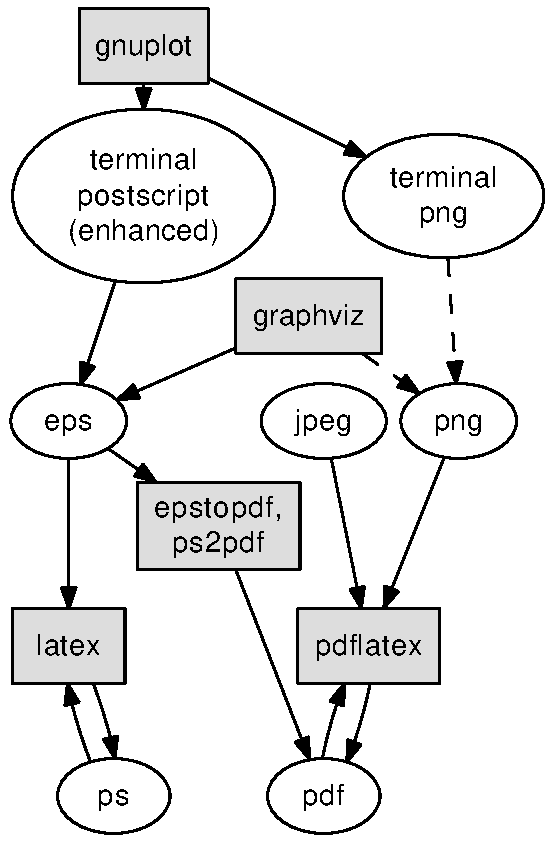
\includegraphics[width=0.4\textwidth]{rys_graf.pdf}
\end{center}
\caption{Przykładowy schemat z graphviz'a. Przerywane strzałki oznaczają, że wszędzie gdzie się da używamy grafiki wektorowej -- unikamy wstawiania bitmap do dokumentu. W niektórych przypadkach użycie bitmap jest uzasadnione (w celu szybkiego podglądu na ekranie lub dla niezwykle skomplikowanych grafik, zawierających np.~setki tysięcy obiektów).}
\label{fig-schemat}
\end{figure}


To jest przykładowy tekst w LaTeX -- pokazuje jak

\begin{tightlist}
\item wstawić schemat stworzony graphviz'em (Rys.~\ref{fig-schemat}),
\item wstawić wykres stworzony gnuplot'em (Rys.~\ref{fig-1Tdelta}, \ref{fig-3d}, \ref{fig-every} i \ref{fig-regr}),
\item zacytować literaturę sformatowaną przez bibtex~\cite{MiOIB,Goldberg-2002},
\item odwoływać się do rysunków, cytowań i części sprawozdania (np.\ rozdział~\ref{sec-eksperymenty}).
\end{tightlist}

Nowsze wersje gnuplota mają już całkiem niezły terminal 'pdf', więc zwykle można zrezygnować z pośrednictwa formatu ps/eps.


\begin{figure}
\begin{center}
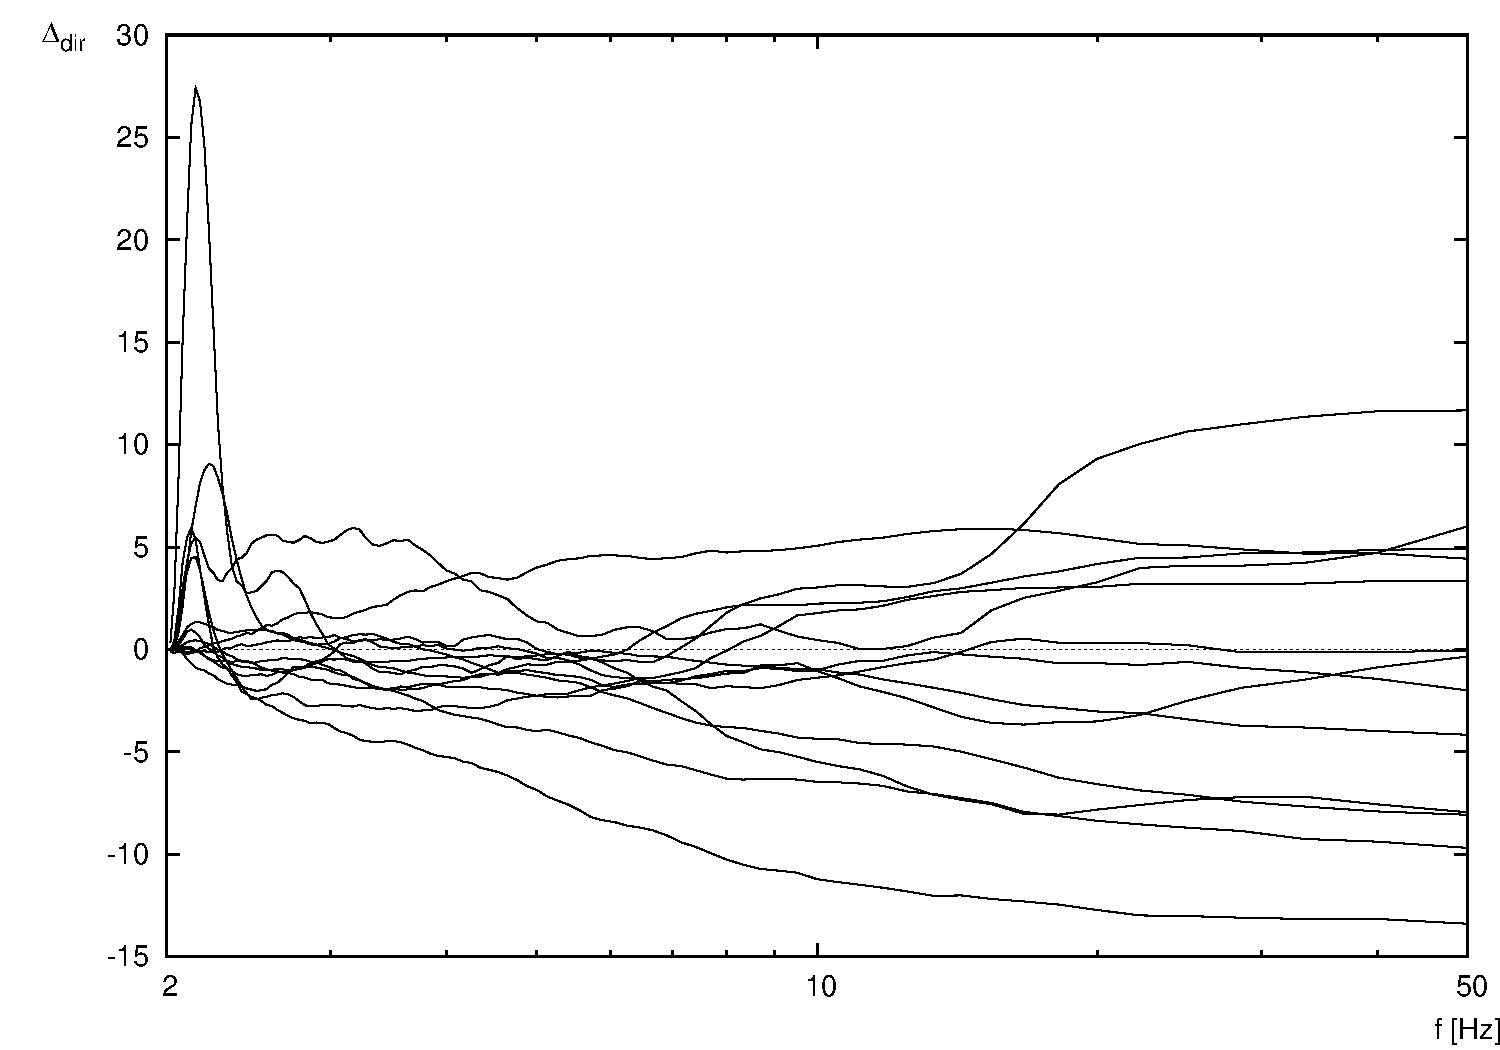
\includegraphics[width=0.8\textwidth]{rys_wykres2d.pdf}
\end{center}
\caption{Przykładowy wykres z gnuplota, terminal postscript, zamieniony na pdf za pomocą programu epstopdf z dystrybucji LaTeX'a (czasem eps2pdf). Różnice $\Delta_{dir}$ wartości $p_{dir}$ dla kąta $90^\circ$.}
\label{fig-1Tdelta}
\end{figure}

\begin{figure}
\begin{center}
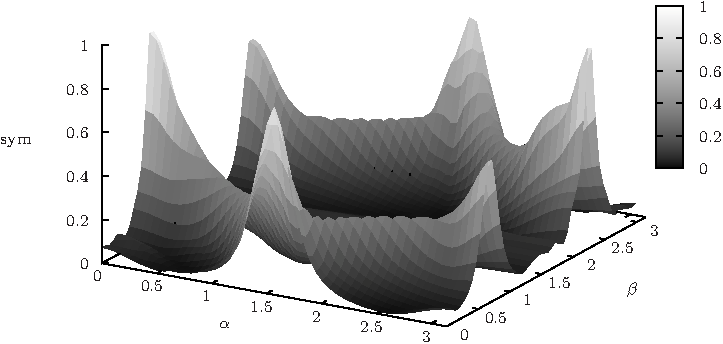
\includegraphics[width=0.9\textwidth]{rys_wykres3d.pdf}
\end{center}
\caption{Jeszcze jeden przykładowy wykres z gnuplota.}
\label{fig-3d}
\end{figure}

\begin{figure}
\begin{center}
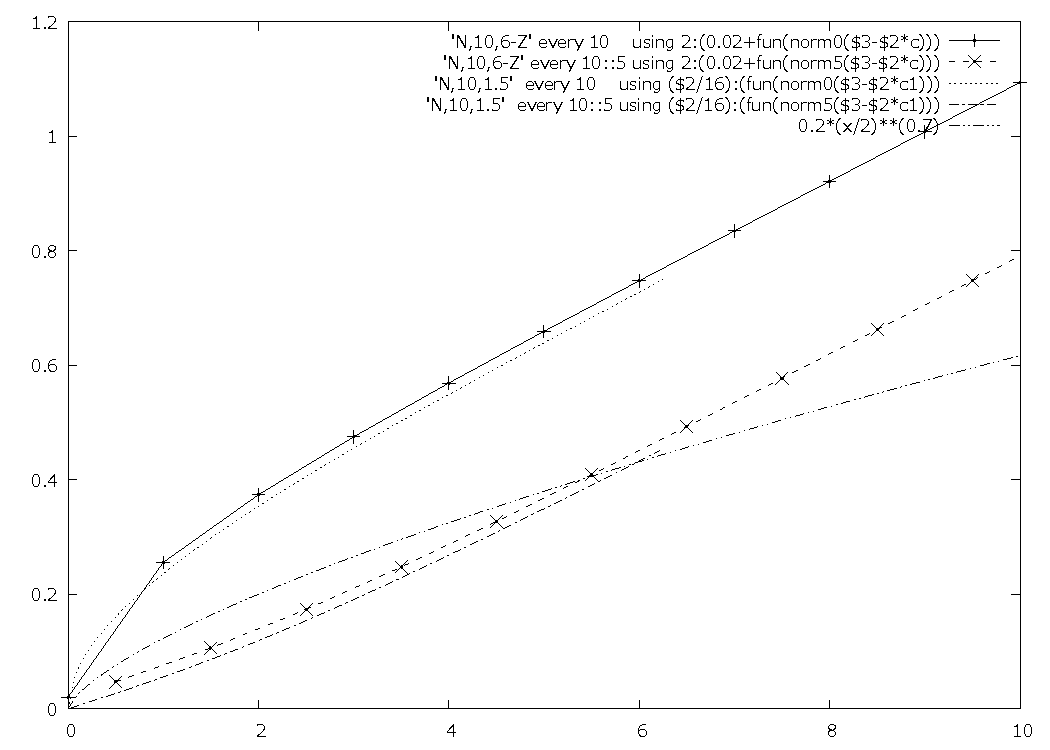
\includegraphics[width=0.85\textwidth]{rys_gnuplot_every.pdf}
\end{center}
\caption{Przykład filtrowania danych do wykresu (\emph{every}) oraz użycie własnych funkcji i formuł w gnuplocie.}
\label{fig-every}
\end{figure}

\begin{figure}
\begin{center}
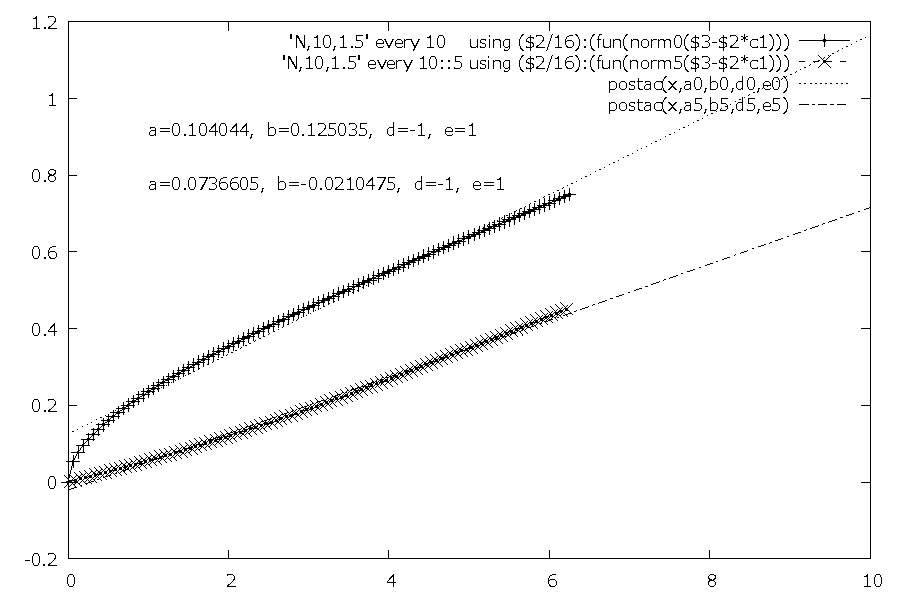
\includegraphics[width=0.85\textwidth]{rys_gnuplot_regr.pdf}
\end{center}
\caption{Przykład regresji: gnuplot ma wbudowany moduł dopasowujący do danych parametry funkcji o dowolnej zadanej postaci. Pozwala też definiować makra, prowadzić obliczenia i umieszczać na wykresie etykiety.}
\label{fig-regr}
\end{figure}

\clearpage %pozwol umiescic zalegle rysunki od razu tutaj 


\section{Eksperymenty}
\label{sec-eksperymenty}

Pamiętajmy o różnicy pomiędzy łącznikiem\footnote{Poszukaj w Wikipedii hasła \emph{Dywiz}.} a myślnikiem, a także o cytowaniu wszelkich materiałów źródłowych w odpowiednich miejscach~\cite{WikiDash}. Cytujmy konkretną stronę, a nie ogólny adres witryny. Cudzysłowy polskie piszmy metodą ,,przecinków i apostrofów''.

Do sprawdzania pisowni bezpośrednio w pliku\ .tex służy między innymi program \emph{aspell}. Rozumie on różne sposoby kodowania polskich literek, a także ma wbudowane filtry do html'a i innych popularnych formatów. Dzięki tym filtrom pomija słowa kluczowe, analizując tylko właściwy tekst.




%%%%%%%%%%%%%%%% literatura %%%%%%%%%%%%%%%%

\bibliography{sprawozd}
\bibliographystyle{plain}


\end{document}

